\begin{frame}{Fitting Non-linear Data}
\begin{itemize}
    \item What if $y$ is a non-linear function of $x$? 
    \item Will this approach still work?
\end{itemize}

\begin{center}
    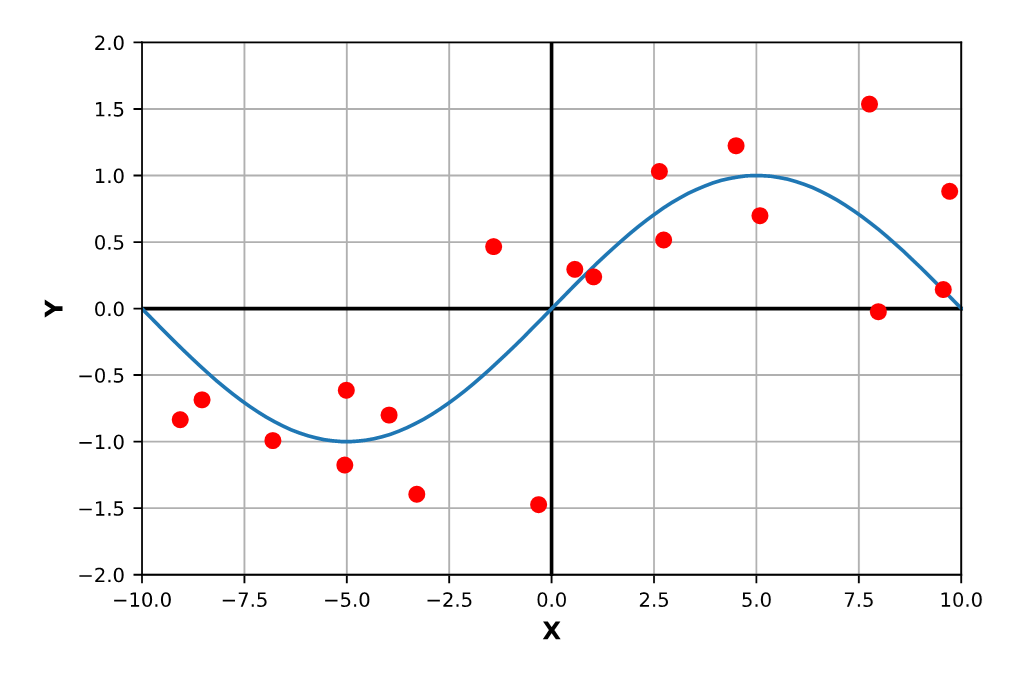
\includegraphics[width=0.75\linewidth]{images/linear-regression/linear-regression-11.png}
\end{center}
\end{frame}


\begin{frame}{Transforming the Feature Space \\ (Feature Engineering)}
\begin{itemize}
    \item We can transform features $x_i$:
\end{itemize}

\[
x_i = \left(x_i^{1}, x_i^{2}, x_i^{3}, \dots, x_i^{m}\right)
\]

\vspace{0.5em}

\begin{itemize}
    \item We will apply some non-linear transformation $\phi$:
\end{itemize}

\[
\phi : \mathbb{R}^m \rightarrow \mathbb{R}^M
\]

\vspace{0.5em}

\begin{itemize}
    \item For example, Polynomial transformation:
\end{itemize}

\[
\phi(x_i) = \left\{ 1, x_i^{1}, x_i^{1,[2]}, \dots, x_i^{1,[k]}, x_i^{2}, x_i^{2,[2]}, \dots, x_i^{2,[k]}, \dots, x_i^{m}, x_i^{m,[2]}, \dots, x_i^{m,[k]} \right\}
\]
\end{frame}


\begin{frame}{Transforming the Feature Space \\ (Feature Engineering)}
\begin{center}
    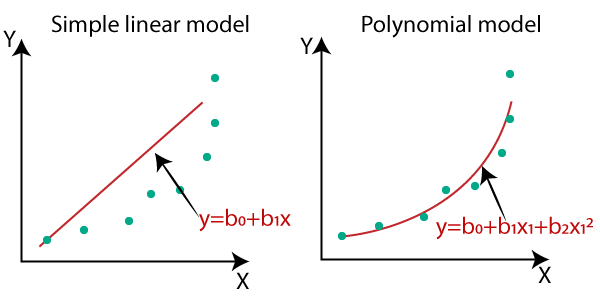
\includegraphics[width=0.9\linewidth]{images/linear-regression/linear-regression-12.png}
\end{center}
\end{frame}


\begin{frame}{Transforming the Feature Space \\ (Feature Engineering)}
\begin{itemize}
    \item \textbf{Example:} Assume you have: 
    \[
    x_i^1: \text{Length} \qquad x_i^2: \text{Width}
    \]
    
    \item You can add \( x_i^3: \text{Area} = x_i^1 \cdot x_i^2 \) to the dataset.
    
    \item \textbf{Other types:}
    \begin{itemize}
        \item Cosine, splines, radial basis functions, etc.
        \item Encoding (Label encoding, One-hot, \dots)
        \item Domain-related features (e.g., financial measures)
        \item Time-related features (Day, month, year, \dots)
        \item Group-level features (e.g., average income per household, total sales per region, median age per team). Often called ``Aggregation features''.
    \end{itemize}
\end{itemize}
\end{frame}
